\chapter{DESIGN AND IMPLEMENTATION}\label{ch:result}

\section{System Architecture Design}

The system architecture described in Chapter \ref{sec:system_architecture} identified four layers: the Web system, the XAI Analysis Layer, the Blockchain Trust Layer, and the Data and Storage Tier. In the implementation, these layers map to a set of concrete software modules organized across two main directories within the project repository.

The first directory, \texttt{block\_chain\_module}, contains the Solidity smart contract ({DocumentRegistry.sol}), the Hardhat configuration and deployment scripts, and the blockchain connector API (\texttt{connector.js}) that provides a JavaScript interface for interacting with the deployed contract.
  \begin{figure}[H]
    \centering

    \begin{minipage}{0.48\textwidth}
        \centering
        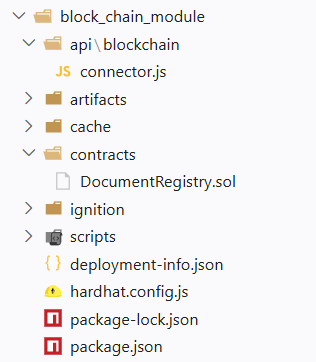
\includegraphics[width=\linewidth]{figures/file_structure_blockchain.png}
        \caption{Blockchain file structure}
        \label{fig:blockchain_file_structure}
    \end{minipage}
    \hfill
    \begin{minipage}{0.48\textwidth}
        \centering
        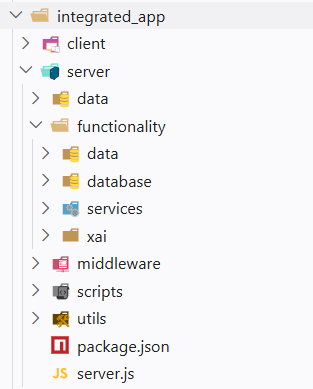
\includegraphics[width=\linewidth]{figures/file_structure_backend.png}
        \caption{Backend file structure}
        \label{fig:backend_file_structure}
    \end{minipage}

\end{figure}

The second directory, \texttt{integrated\_app}, contains the Express.js backend server (\texttt{server.js}), the XAI analysis modules (under \texttt{functionality/xai/}), the database handlers (under {functionality/database/}), the service modules for chunking, embedding, OCR, and field extraction (under \texttt{functionality/services/}), the document parser utility (under \texttt{utils/}), the authentication middleware (under \texttt{middleware/}), and the Next.js frontend client (under \texttt{client/}).

\subsection{How Components Communicate}

The four architectural layers communicate through well-defined interfaces, each using the communication protocol best suited to its requirements:

\begin{itemize}
    \item \textbf{Frontend to Backend (HTTP/JSON):} The Next.js frontend communicates with the Express.js backend through RESTful HTTP endpoints. All requests and responses use JSON formatting. For document uploads, the frontend sends \texttt{multipart/form-data} requests that include both the file binary and any associated metadata fields. The backend responds with structured JSON objects containing the verification results, blockchain transaction data, and XAI explanations.
    
    \item \textbf{Backend to Blockchain (JSON-RPC):} The backend server communicates with the Ethereum node through JSON-RPC, an asynchronous remote procedure call protocol. The {BlockchainConnector} class uses the \texttt{ethers.js} library to construct and submit transactions. This asynchronous design ensures that blockchain operations which require network confirmation do not block the Express.js event loop or delay responses to other API requests.
    
    \item \textbf{Backend to XAI Module (Internal Function Calls):} The XAI analysis modules are integrated directly into the Node.js process as imported JavaScript modules. The backend server invokes analysis functions through direct method calls on singleton instances (e.g., {xaiAnalyzer.analyzeDocument(filePath, metadata)}). This approach eliminates network overhead and simplifies error handling, as exceptions propagate naturally through the call stack.
    
    \item \textbf{Backend to Database (SQL over TCP):} The backend communicates with the Neon PostgreSQL database through the \texttt{pg} (node-postgres) library, which manages a connection pool for concurrent query execution. For vector similarity searches, the backend constructs SQL queries that use the \texttt{pgvector} operator (\texttt{<=>}) to compute cosine distances between embedding vectors directly within the database engine.
\end{itemize}

\subsection{Development Environment}

The system was developed and tested on a Ubuntu operating system, using Node.js v24+, Hardhat with Solidity 0.8.24, and Neon PostgreSQL with the \texttt{pgvector} extension enabled. The Hardhat local network runs on the developer's machine at \texttt{http://127.0.0.1:8545} to simulate Ethereum interactions without testnet gas costs. These specifications are listed to support the reproducibility of the experimental results presented in Chapter 5.

\section{Module Design}

This section describes the implementation of each major module, progressing from the user-facing frontend through the backend orchestrator to the specialized analysis and storage services.

\subsection{Frontend Module Design}

The frontend client is a Next.js web application that provides the user interface for document submission and result viewing. Next.js was selected for its server-side rendering capabilities, file-system-based routing, and built-in performance optimizations. The frontend is organized into a component-based architecture where each user interaction is handled by a dedicated component.

The document upload component supports multiple file formats including PDF, DOCX, and image files. Before transmitting a file to the backend, the component performs client-side validation to check file size (maximum 50 MB for documents, 10 MB for certificate verification) and file type constraints. If the validation fails, the user receives an immediate error message without consuming server resources. Upon successful upload, the component receives a unique document identifier from the backend, which is used to track the verification progress.

\begin{figure}[H]
    \centering
    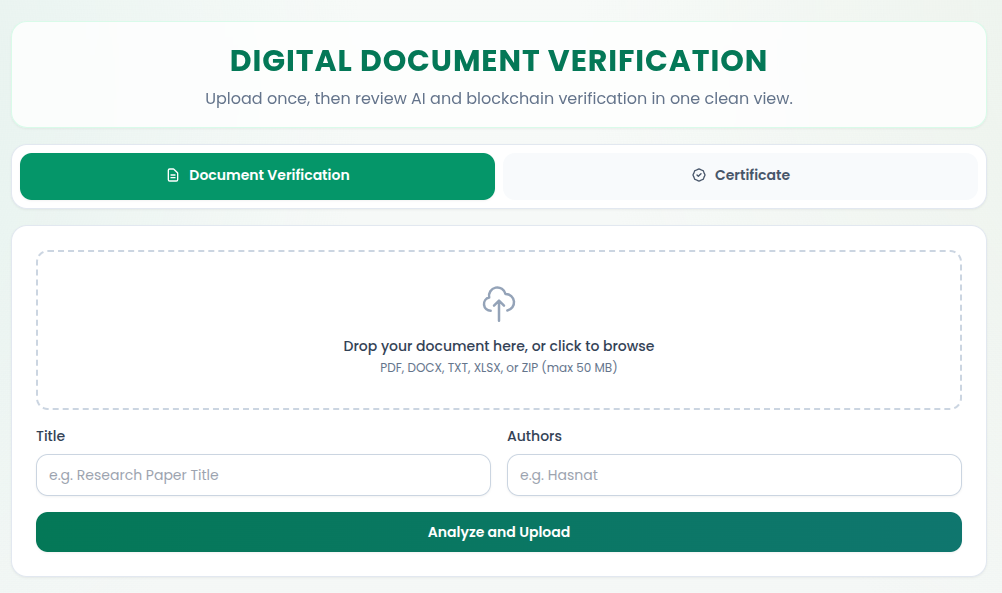
\includegraphics[width=0.95\linewidth]{figures/UI/initial_paper_verification_UI.png}
    \label{Article or Journal paper verification UI}
    \caption{Article or journal paper verification UI}
\end{figure}

The verification result component renders the multi-layered analysis output returned by the backend. For large-document verification, this includes the overall verdict (Verified or Rejected), the confidence score, the plagiarism similarity map with per-section match details, the AI detection indicators, and the blockchain transaction receipt. For certificate verification, the component displays the field-by-field comparison table (showing expected versus found values for each canonical field), the forgery risk assessment, and the blockchain anchoring status.

The system supports two distinct verification interfaces. The first is designed for research papers and journal articles, where users upload a document and the system checks it against the existing corpus for plagiarism and AI-generated content. The second is designed for certificates, where issuing organizations register credentials and verifiers upload copies to check authenticity.

\begin{figure}[H]
    \centering
    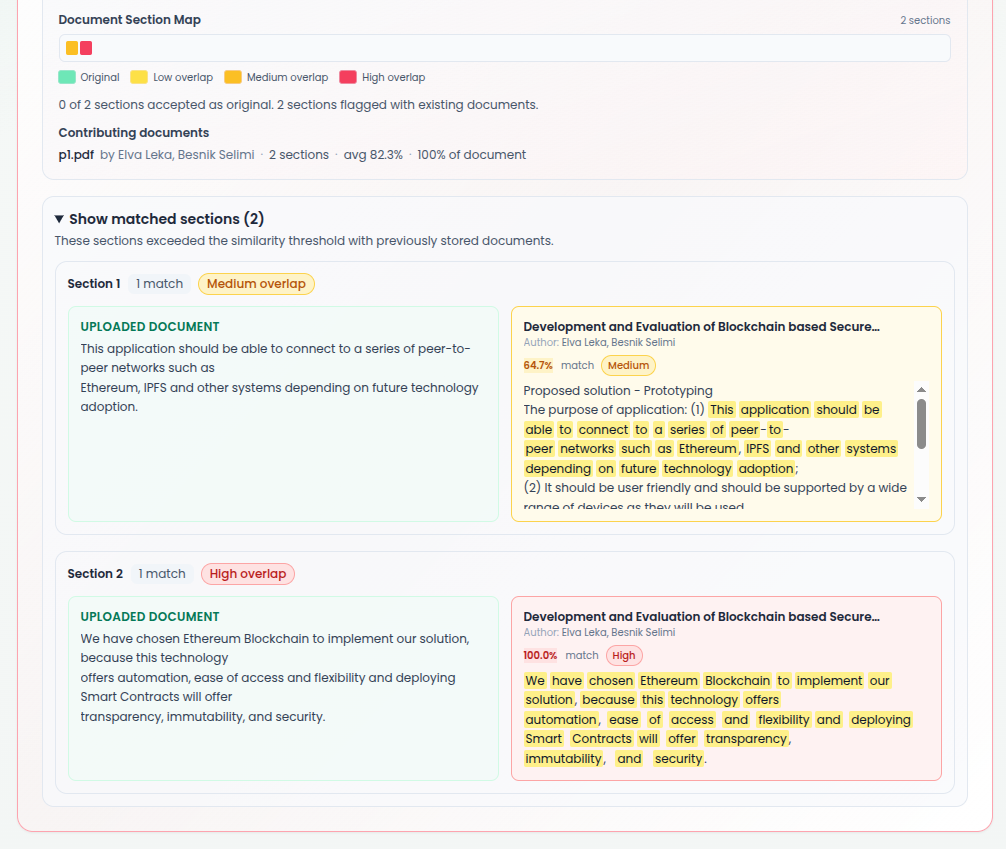
\includegraphics[width=0.9\linewidth]{figures/UI/rejected_paper_ui_2.png}
    \label{Article or Journal paper verification UI}
    \caption{Explaining why an article was rejected by showing matching documents.}
\end{figure}


\subsection{Backend Application Server Module}

The backend application server is the central orchestrator of the system, implemented as a single Express.js application in \texttt{server.js}. The server handles request routing, file upload management, service initialization, and workflow coordination across all other modules.
\begin{itemize}
\item \textbf{Middleware Stack:} The server configures a layered middleware stack that processes every incoming request. The CORS middleware enables cross-origin requests from the frontend application. The \texttt{express.json()} middleware parses JSON request bodies. For file uploads, the server uses the Multer middleware library, which handles \texttt{multipart/form-data} parsing and stores uploaded files to disk. Three separate Multer configurations are defined, each with different file size limits and accepted MIME types:

\begin{itemize}
    \item The primary upload configuration accepts documents up to 50 MB in formats including PDF, DOCX, TXT,  Markdown.
    \item The small-document upload configuration accepts PDF and image files (PNG, JPEG, WebP) up to 10 MB.
    \item The certificate upload configuration accepts PDF and image files up to 10 MB and stores files in a dedicated \texttt{certificates} subdirectory with timestamped filenames to prevent naming collisions.
\end{itemize}

\item \textbf{Service Initialization:} When the server starts, the \texttt{initializeServices()} function executes a sequential initialization sequence. First, the database handler connects to the Neon PostgreSQL instance and creates any missing tables. Second, the chunking service is initialized with a reference to the database handler. Third, the blockchain connector tests its connection to the Hardhat node by querying the total document count. If any service fails to initialize, the server logs a warning but continues running, allowing partial functionality when some services are temporarily unavailable.

\item \textbf{Error Handling:} The server implements structured error handling at both the middleware and endpoint levels. Each API endpoint wraps its logic in a try-catch block. When an error occurs, the server logs the full error stack to the console and returns a JSON response with a \texttt{success: false} flag, a human-readable error message, and (in development mode) the stack trace. For file upload errors or rejections, the server deletes the temporarily uploaded file before returning the error response, preventing disk space accumulation from rejected or failed uploads.
\end{itemize}

\subsection{Explainable AI Module}

The XAI module is implemented as the \texttt{RealXAIAnalyzer} class in {functionality/xai/real-analyzer.js}. This class encapsulates all three diagnostic tests described in Chapter \ref{sec:Explainable AI} and the result combination logic described in Chapter \ref{sec:result_comb_score}. The class is instantiated as a singleton and exported for use by the server.

\textbf{Document Analysis Pipeline:} The main entry point is the \texttt{analyzeDocument(filePath, metadata)} method, which orchestrates the following sequence:

\begin{enumerate}
    \item \textbf{Hash Computation:} The method calls \texttt{calculateHash(filePath)}, which streams the file through Node.js's \texttt{crypto.createHash('sha256')} and produces the \texttt{0x}-prefixed hexadecimal digest.
    \item \textbf{Text Extraction:} The method calls \texttt{extractText(filePath)}, which delegates to the \texttt{DocumentParser} module. If the parser returns empty text (for example, from a scanned image without OCR), the method falls back to using the filename as a minimal text representation.
    \item \textbf{Plagiarism Check:} The method calls \texttt{runPlagiarismCheck(filePath, documentText)}, which normalizes the text, constructs 8-word n-gram shingles using the {buildNGrams(words, 8)} method, counts shingle frequencies, and computes a similarity score based on the ratio of duplicate shingles to total shingles. The similarity score is computed by multiplying the duplicate shingle ratio (a value between 0 and 1) by 180 and capping the result at 100. This amplification factor ensures that even modest internal duplication rates produce noticeable scores; for example, a duplicate ratio of 0.42 (42\% of shingles repeated) yields a score of 75.6, which triggers the plagiarism threshold. Documents with fewer than 40 words are skipped with a score of 0, as they do not contain enough text for reliable analysis.
    \item \textbf{AI Detection:} The method calls \texttt{runAIDetection(filePath, documentText)}, which computes five linguistic indicators as described in Chapter \ref{sec:text_extraction_normalization}. The implementation uses the \texttt{splitSentences(text)} method for sentence-boundary detection (splitting on \texttt{.}, \texttt{!}, and \texttt{?}), the \texttt{variance(values)} method for computing statistical variance, and the \texttt{repeatedSentenceRatio(sentences)} method for measuring sentence repetition. Documents with fewer than 50 words or fewer than 3 sentences are assigned a default low probability of 20\%.
    \item \textbf{Certificate Forgery Check:} If the metadata indicates the document is a certificate, the method calls \texttt{runCertificateForgeryCheck(filePath, documentText)}, which performs the four structural signal checks described in Chapter \ref{sec:cryptographic_fingerprint_sha256}.
    \item \textbf{Result Combination:} The method calls \texttt{combineResults(...)}, which implements the confidence scoring logic described in Chapter \ref{sec:result_comb_score}. The output includes the document hash, overall status, confidence score, individual analysis results, rejection reasons (if any), and the human-readable explanation generated by \texttt{generateExplanation(status, rejectionReasons, results)}.
\end{enumerate}

The \texttt{generateExplanation} method produces a structured explanation object containing a summary statement, an array of detailed findings (each prefixed with a check mark or cross mark), and a recommendation. For verified documents, the explanation lists all passed checks with their scores. For rejected documents, it lists each issue type (plagiarism, AI-generated, or forgery) with the specific evidence that triggered the rejection.

\subsection{Vector Embedding Service}

The vector embedding pipeline is implemented across two modules: \texttt{EmbeddingService} for vector generation and \texttt{ChunkingService} for text segmentation and similarity search orchestration.
\begin{itemize}
    
\item \textbf{Embedding Generation:} The \texttt{EmbeddingService} class (in {functionality/services/embedding-service.js}) uses the \texttt{@xenova/transformers} library to load the \texttt{Xenova/all-MiniLM-L6-v2} sentence transformer model. The model is loaded lazily on the first invocation and cached for subsequent calls through a promise-based singleton pattern. The \texttt{embedText(text)} method passes the input text through the model's feature-extraction pipeline with mean pooling and L2 normalization, producing a 384-dimensional float array. The normalization ensures that cosine similarity can be computed as a simple dot product.

\item \textbf{Text Chunking:} The \texttt{ChunkingService} class (in {functionality/services/chunking-service.js}) segments document text into sentence-level chunks. The segmentation proceeds in two stages. First, the \texttt{stripReferencesSection(text)} method removes the references and bibliography section using a two-strategy detection approach. The primary strategy searches for explicit section headers (matching against 15 header variations including "References," "Bibliography," "Works Cited," and "Literature Cited") using a regular expression that accounts for numbered prefixes, Roman numeral prefixes, and trailing punctuation. If no header is found, the fallback strategy scans the latter half of the document for runs of three or more consecutive lines that contain citation markers (such as \texttt{[1]}, \texttt{(1)}, or inline DOI references with publication years). Second, the \texttt{splitIntoChunks(text)} method splits the remaining text at sentence-ending punctuation marks (\texttt{.}, \texttt{!}, \texttt{?}) and returns an array of chunk objects, each containing the text content, chunk index, and character length.

\item \textbf{Similarity Search:} The \texttt{findSimilarChunks(queryText, documentId, threshold)} method implements the cross-document similarity search described in Chapter \ref{sec:Cert_forgery_isolation}. The method first checks whether the query is a DOI reference or too short (fewer than 5 tokens), skipping such queries to avoid false positives. It then generates an embedding vector for the query text and passes it to the PostgreSQL handler's {searchSimilarChunksByEmbedding} method, which executes a SQL query using the \texttt{pgvector} cosine distance operator (\texttt{<=>}). The query computes \texttt{(1 - cosine\_distance)} as the similarity score and returns all chunks above the threshold (default: 0.25), ordered by similarity.

\item \textbf{Hybrid Scoring:} In the main document upload workflow (implemented in \texttt{server.js}), the system extends the pure embedding similarity with a hybrid scoring approach. For each uploaded chunk, the system first retrieves embedding-similar candidates from the database (threshold: 0.4). For candidates with embedding similarity above 0.7, the system additionally computes a phrase-overlap score using the \texttt{calculatePhraseOverlap} function, which splits both texts by punctuation boundaries into segments, normalizes each segment (lowercase, strip list markers, collapse whitespace), and computes the fraction of uploaded segments that appear in the database text. The final hybrid score is computed as a weighted average: $$0.5 \times \text{embeddingScore} + 0.5 \times \text{phraseOverlapScore}$$ A document is rejected if the average hybrid score across all chunks exceeds 40\%.
\end{itemize}

\subsection{Document Parser}

The \texttt{DocumentParser} class (in \texttt{utils/document-parser.js}) implements the multi-format text extraction outlined in Chapter \ref{sec:text_extraction_normalization}. The implementation-specific details of this extraction include using \texttt{pdf-parse/lib/pdf-parse.js} directly (bypassing the default entry point to avoid a debug-mode side effect that writes to disk), falling back to the \texttt{pdftotext} command-line utility with \texttt{-q -layout} flags for complex PDFs, and employing regular expressions to strip RTF control sequences (\texttt{\{\textbackslash\textbackslash...\}}) when parsing Rich Text Format documents. The remaining formats are processed using the specific Node.js libraries described in the methodology.

\section{Database Design}

The database system was designed to support all four data categories described in Chapter \ref{sec:Neon_database}: document records, sentence-level chunks, certificate records, and organization records. The implementation uses Neon PostgreSQL with the \texttt{pgvector} extension enabled for native vector similarity search.

The database schema is managed by the \texttt{PostgreSQLHandler} class (in {functionality/database/postgres-handler.js}), which creates and maintains five tables. The connection is established using the \texttt{pg} (node-postgres) library with a connection pool, using the \texttt{DATABASE\_URL} environment variable that follows the Neon connection string format. For cloud connections, SSL is enabled with \texttt{rejectUnauthorized: false} to support Neon's serverless endpoint.

\textbf{Table 1 --- documents:} Stores metadata for uploaded documents. Key columns include \texttt{id} (auto-incrementing primary key), \texttt{filename} (original file name), \texttt{doc\_hash} (SHA-256 hash with a unique constraint for deduplication), \texttt{metadata} (JSONB column storing XAI results, blockchain data, uploader name, document type, and status), \texttt{title}, \texttt{authors}, and \texttt{uploaded\_at} (timestamp).

\textbf{Table 2 --- chunks:} Stores sentence-level text chunks for similarity search. Key columns include \texttt{document\_id} (foreign key to documents), \texttt{chunk\_index} (position within the document), \texttt{chunk\_text} (the sentence content), \texttt{chunk\_hash} (SHA-256 hash of the chunk content, with a unique constraint), \texttt{token\_count}, \texttt{embedding} (JSONB array storing the 100-dimensional word-frequency embedding), and \texttt{embedding\_vector} (a \texttt{vector(384)} column storing the dense transformer embedding for \texttt{pgvector} queries). The \texttt{chunk\_hash} unique constraint serves a dual purpose: it prevents duplicate chunk storage and enables exact-match chunk lookups.

\textbf{Table 3 --- organizations:} Stores issuing organization records. Key columns include \texttt{org\_id} (unique identifier), \texttt{name}, \texttt{api\_key\_hash} (SHA-256 hash of the API key, indexed for fast lookups), \texttt{api\_key\_prefix} (first 12 characters of the API key for identification), \texttt{contact\_email}, \texttt{is\_active} (boolean flag for enabling/disabling organizations), and \texttt{created\_at}.

\textbf{Table 4 --- certificates:} Stores issued certificate records. Key columns include \texttt{certificate\_id} (unique identifier in the format \texttt{CERT-\{timestamp\}-\{random\}}), \texttt{org\_id} (foreign key to organizations), \texttt{issuer\_name}, \texttt{recipient\_name}, \texttt{course\_or\_title}, \texttt{issue\_date}, \texttt{certificate\_serial} (unique within each organization, enforced by a composite unique constraint on \texttt{org\_id} and \texttt{certificate\_serial}), \texttt{canonical\_fingerprint} (SHA-256 hash of the normalized canonical fields), \texttt{file\_hash}, \texttt{document\_data} (BYTEA column storing the original certificate binary), \texttt{document\_mime}, \texttt{ocr\_text}, \texttt{ocr\_engine}, \texttt{ocr\_confidence}, \texttt{blockchain} (JSONB column storing the blockchain transaction receipt), \texttt{status} (active or revoked), \texttt{revoked\_at}, and \texttt{revocation\_reason}. Indexes are created on \texttt{canonical\_fingerprint}, \texttt{file\_hash}, {certificate\_serial}, and \texttt{org\_id} to optimize the multi-strategy matching queries.

\textbf{Table 5 --- small\_documents:} Stores small-format credential records that follow the metadata-fingerprint verification model. Key columns include \texttt{issued\_document\_id}, \texttt{doc\_type}, \texttt{issuer\_name}, \texttt{file\_hash}, \texttt{metadata} (JSONB), \texttt{metadata\_fingerprint}, \texttt{analysis} (JSONB storing the forgery analysis results), and \texttt{blockchain} (JSONB storing the blockchain transaction receipt). Indexes are created on \texttt{file\_hash} and \texttt{issued\_document\_id}.

The full SQL schema implementation is provided in Appendix \ref{appendix:database}.

\section{Blockchain Setup}

The blockchain layer is implemented using the Hardhat development framework, which provides a local Ethereum Virtual Machine (EVM) for testing and development, along with compilation, deployment, and testing tools for Solidity smart contracts.

\subsection{Network Configuration and Node Management}

The Hardhat configuration (in \texttt{block\_chain\_module/hardhat.config.js}) defines two network targets:

\textbf{Development Network (hardhat):} Configured with chain ID 1337 and automatic mining enabled with an interval of 0, meaning each transaction is mined immediately into its own block. This eliminates confirmation delays during development and testing.

\textbf{Localhost Network:} Configured to connect to a persistent Hardhat node running at \\{http://127.0.0.1:8545} with the same chain ID of 1337. This configuration is used when the backend server needs to interact with a long-running blockchain instance that persists state across multiple server restarts.

The Solidity compiler is configured to version 0.8.24 with the optimizer enabled (200 runs), which reduces the gas cost of frequently called functions. The compiled contract artifacts (ABI and bytecode) are stored in the \texttt{artifacts/contracts/} directory and are read by the \texttt{BlockchainConnector} at initialization time.

\subsection{Transaction Management}

The \texttt{BlockchainConnector} class (in \texttt{block\_chain\_module/api/blockchain/connector.js}) manages all interactions between the backend server and the deployed smart contract. The class follows a singleton pattern and lazy initialization: the blockchain connection is established on the first API call and reused for all subsequent calls.
\begin{itemize}
    
\item \textbf{Initialization Sequence:} The \texttt{initialize()} method performs three steps. First, it reads the deployment information (contract address) from \texttt{deployment-info.json}, which is generated by the deployment script. Second, it creates a JSON-RPC provider pointing to the local Hardhat node at \texttt{http://127.0.0.1:8545} and obtains a signer from the first account managed by the node. Third, it loads the compiled contract ABI from the artifacts directory and creates an \texttt{ethers.Contract} instance bound to the contract address, ABI, and signer.

\item \textbf{Transaction Execution:} When the backend server calls \texttt{registerDocument(...)}, the connector executes three sequential on-chain transactions as described in Chapter 3.5.2. Each transaction call follows the pattern: (1) invoke the contract function, which returns a pending transaction object; (2) call \texttt{tx.wait()} to block until the transaction is mined and a receipt is returned; (3) extract the gas consumption from the receipt for performance tracking. The connector converts the SHA-256 hash to a \texttt{bytes32} value by prepending \texttt{0x} if it is not already present.

\item \textbf{Verification Queries:} The \texttt{verifyDocument(documentHash)} method performs read-only queries that do not consume gas. It first calls \texttt{contract.documentExists(hashBytes32)} to check for the hash's presence, and if found, calls \texttt{contract.getDocument(hashBytes32)} to retrieve the full document record including the verification status, XAI analysis summary, confidence score, and registration timestamp.

\item \textbf{Status and Statistics:} The \texttt{getStatus()} method returns the current blockchain connection state, including the contract address, network name, chain ID, total registered documents, and signer address. The \texttt{getStats()} method iterates over registered document hashes (up to 100) and categorizes them by verification status (verified, pending, or rejected).
\end{itemize}

\section{Smart Contract Implementation}

The \texttt{DocumentRegistry} smart contract (in \texttt{block\_chain\_module/contracts/DocumentRegistry.sol}) is the on-chain component of the system. It is written in Solidity 0.8.24 and compiled using the Hardhat toolchain.

\subsection{DocumentRegistry Contract}

The contract defines a \texttt{Document} struct with eight fields that store the complete verification record. The Solidity implementation of this struct is as follows:

\begin{verbatim}
struct Document {
    bytes32 documentHash;
    string documentName;
    address uploader;
    uint256 timestamp;
    bool isVerified;
    string xaiAnalysis;
    string verificationStatus;
    uint256 confidenceScore;
}
\end{verbatim}

The contract uses two storage structures: a \texttt{mapping(bytes32 => Document)} for constant-time lookups by document hash, and a \texttt{bytes32[]} array for iterating over all registered document hashes (used by the statistics endpoint).

The contract exposes six functions:

\begin{enumerate}
    \item \textbf{\texttt{registerDocument(bytes32 \_documentHash, string \_documentName)}:} Creates a new document record with "pending" status. Three \texttt{require} guards enforce invariants: the hash must not already exist (preventing duplicate registrations), the hash must not be zero, and the document name must not be empty. Emits a \texttt{DocumentRegistered} event.
    \item \textbf{\texttt{addXAIAnalysis(bytes32 \_documentHash, string \_xaiAnalysis)}:} Attaches the XAI analysis summary to an existing document. Requires the document to exist and the analysis string to be non-empty. Emits an \texttt{XAIAnalysisAdded} event.
    \item \textbf{\texttt{verifyDocument(bytes32 \_documentHash, bool \_isVerified, string \_verificationStatus, uint256 \_confidenceScore)}:} Updates the verification status of an existing document. Requires the document to exist, the confidence score to be between 0 and 100, and the status string to be non-empty. Emits a \texttt{DocumentVerified} event.
    \item \textbf{\texttt{getDocument(bytes32 \_documentHash)}:} Returns all eight fields of a document record. This is a \texttt{view} function (no gas cost for external calls). Requires the document to exist.
    \item \textbf{\texttt{documentExists(bytes32 \_documentHash)}:} Returns a boolean indicating whether a document hash has been registered. This is a \texttt{view} function.
    \item \textbf{\texttt{getVerificationStatus(bytes32 \_documentHash)}:} Returns only the verification-related fields (\texttt{isVerified}, \texttt{verificationStatus}, \texttt{confidenceScore}). This lightweight query is used for quick status checks without transferring the full document record.
\end{enumerate}

Additionally, \texttt{getTotalDocuments()} returns the length of the document hashes array, and \texttt{getDocumentHashByIndex(uint256 \_index)} enables sequential traversal of all registered documents.

The complete Solidity implementation is provided in Appendix \ref{appendix:code-verify_document_in_blockchian}.

\subsection{On-Chain Data Minimization}

A critical design decision was to minimize the data stored on-chain. Blockchain storage is expensive (approximately 20,000 gas per 256-bit word in Ethereum), and storing full analysis reports would make the system impractical. The implementation addresses this by storing only a compact JSON summary in the \texttt{xaiAnalysis} field. This summary includes the overall status, similarity score, AI probability, and match count---typically under 200 bytes. The complete analysis report, including all matched sections, per-section similarity scores, and full XAI explanations, is stored in the PostgreSQL database. The SHA-256 hash serves as the link between the on-chain proof and the off-chain details.

\section{Document Hashing Process}

The document hashing implementation realizes the cryptographic fingerprinting methodology.

\subsection{SHA-256 Hash Computation}

The hash computation is implemented as a streaming operation using Node.js's built-in \texttt{crypto} module. The \texttt{calculateFileHash(filePath)} function creates a read stream from the file, pipes the data through \texttt{crypto.createHash('sha256')}, and returns the hexadecimal digest prefixed with \texttt{0x}. The streaming approach ensures that large files (up to 50 MB) are processed without loading the entire file into memory, which is essential for server environments with limited RAM.

The same hashing algorithm is used at multiple points in the system: during initial upload (for deduplication), during blockchain registration (as the on-chain identifier), and during verification (for hash comparison against stored records). The consistency of the algorithm across all stages ensures that any tampering at any point will produce a mismatch.

\subsection{Hash Integrity Implementation}

The security properties of SHA-256 were discussed in Chapter \ref{sec:cryptographic_fingerprint_sha256}, including its collision resistance ($2^{128}$ birthday bound) and preimage resistance ($2^{256}$). In the implementation, these properties are leveraged at three distinct points: during initial upload (for deduplication against the database), during blockchain registration (as the on-chain document identifier), and during third-party verification (for hash comparison against stored records). The consistent use of the same algorithm at all three stages ensures that any document modification, however small, is detected as a hash mismatch at every layer.

\subsection{Hash-Based Document Deduplication}

The system implements a three-layer deduplication strategy using document hashes:

\begin{enumerate}
    \item \textbf{Blockchain Layer:} Before any new registration, the backend queries {blockchainConnector.verifyDocument(hash)} to check if the hash already exists on-chain. If it does, the upload is immediately rejected with a detailed error response indicating the existing document's name and registration timestamp.
    \item \textbf{Database Layer:} If the blockchain check passes (or is unavailable), the backend queries \texttt{dbHandler.getDocumentByHash(hash)} to check the PostgreSQL documents table. If a record with the same hash exists, the upload is rejected.
    \item \textbf{Certificate Layer:} For certificate issuance, the system additionally calls \\{dbHandler.findCertificateByFileHash(hash)} to prevent duplicate certificate registrations even when the document table check passes (since certificates are stored in a separate table).
\end{enumerate}

This layered approach ensures that no duplicate document is ever registered, regardless of which storage layer receives the first copy.

\section{Certificate Issuance and Verification Implementation}

The certificate management subsystem implements the methodology through two primary API endpoints: one for issuance and one for verification.

\subsection{Certificate Issuance Flow}

When an authorized organization issues a certificate through the \texttt{POST /api/certificates/issue} endpoint, the system executes the following sequence:

\begin{enumerate}
    \item \textbf{Authentication:} The \texttt{requireOrgAuth} middleware validates the \texttt{X-Org-API-Key} header by hashing the provided key with SHA-256 and looking up the hash in the organizations table. If the key is valid and the organization is active, the request proceeds with the organization's identity attached to \texttt{req.org}.
    \item \textbf{Payload Parsing:} The \texttt{parseCanonicalPayload(body)} function extracts the five canonical fields (recipient name, course or title, issue date, certificate serial, and additional fields) from the request body. Missing dates default to the current date in ISO format.
    \item \textbf{Duplicate Detection:} The system checks for duplicate certificates by serial number (within the same organization) and by file hash (globally). If either check finds an existing record, the request is rejected with a 409 Conflict response.
    \item \textbf{OCR Processing:} The uploaded certificate file is passed to {ocrService.extractText(filePath)}, which uses Tesseract for image files or \texttt{pdf-parse} for PDF files.
    \item \textbf{Canonical Fingerprint Generation:} The {fieldExtractor.buildCanonicalFingerprint(canonicalFields)} function sorts the field names, normalizes the values, and computes a SHA-256 hash of the resulting JSON string.
    \item \textbf{Blockchain Anchoring:} The system calls \texttt{blockchainConnector.registerDocument(...)} with the file hash, a certificate-specific document name, a JSON summary of the issuance metadata (including the canonical fingerprint, a hash of the recipient name, the issue date, and the serial number), and a confidence score of 95.
    \item \textbf{Database Storage:} The certificate record is saved to the certificates table with all canonical fields, the file hash, the canonical fingerprint, the original document binary (as BYTEA), the OCR text, the blockchain transaction receipt, and an "active" status.
    \item \textbf{QR Code Generation:} The response includes a QR code payload containing the certificate ID, issuer name, recipient name, file hash, and a verification URL. The QR code image is generated dynamically using an external QR code API.
\end{enumerate}

\subsection{Certificate Verification Flow}

When a user verifies a certificate through the \texttt{POST /api/certificates/verify} endpoint, the system implements the multi-strategy matching and field-level comparison:

\begin{enumerate}
    \item \textbf{Hash Computation and OCR:} The uploaded file's SHA-256 hash is computed, and OCR is performed to extract text.
    \item \textbf{Field Extraction:} The \texttt{fieldExtractor.extractAllFields(ocrText)} function applies the library of regular expression patterns to identify the five canonical fields. The \\\texttt{fieldsToCanonical(fields)} function converts the extraction results into a canonical form, and \texttt{buildCanonicalFingerprint(canonical)} computes the fingerprint.
    \item \textbf{Multi-Strategy Matching:} The system attempts to find a matching certificate record through four strategies in order: (a) hint certificate ID from the request body, (b) file hash match, (c) extracted or hinted serial number match, and (d) canonical fingerprint match.
    \item \textbf{Field Comparison:} The \texttt{fieldExtractor.compareFields(stored, extracted)} function performs the field-by-field comparison. The \texttt{fieldMatchStatus(expected, found)} function determines the match status for each field using normalized string comparison, whitespace-insensitive comparison, word-level overlap analysis, and fuzzy partial matching (60\% word overlap threshold). For date fields, the {isDateMatch(storedDate, extractedDate)} function generates multiple format variants (ISO, DD/MM/YYYY, natural language) and compares normalized versions.
    \item \textbf{Verdict Assignment:} The verdict is determined by a decision tree: if the certificate is revoked, the verdict is "revoked"; if the file hash matches, the verdict is "authentic"; if any field has a mismatch status, the verdict is "tampered"; if the matched record was found and at least three fields match exactly, the verdict is "authentic"; otherwise, the verdict is "suspicious."
    \item \textbf{XAI Report Generation:} The \texttt{buildXaiAnalysis(...)} function constructs a detailed XAI report for each verdict, including structured reasons (positive, critical, warning, or info), evidence items (field differences with their expected and found values), and actionable recommendations. Each verdict type generates a distinct confidence score: authentic (95\%), revoked (99\%), tampered (90\%), not-a-certificate (85\%), suspicious (60\%), and unknown (30\%).
    \item \textbf{Blockchain Re-Anchoring:} If the certificate record exists in the database but is not found on the current blockchain instance (for example, after a Hardhat node restart), the system automatically re-anchors it by executing a new blockchain registration transaction and updating the certificate's blockchain metadata in PostgreSQL.
\end{enumerate}

\section{REST API Endpoint Design}

The backend server exposes a set of RESTful API endpoints that serve as the interface between the frontend client and the backend services.

\begin{table}[hbt!]
\centering
\caption{Primary API Endpoints}
\renewcommand{\arraystretch}{1.2}

\begin{tabularx}{\textwidth}{|p{1.5cm}|X|p{3.5cm}|p{2.5cm}|}
\hline
\textbf{Method} & \textbf{Endpoint} & \textbf{Description} & \textbf{Authentication} \\ 
\hline

GET & \texttt{/api/health} & Health check and service status & None \\ \hline

GET & \texttt{/api/blockchain/status} & Blockchain connection status and statistics & None \\ \hline

POST & \texttt{/api/document/upload} & Upload and analyze a document (full pipeline) & None \\ \hline

GET & \texttt{/api/document/:id} & Retrieve document details by ID & None \\ \hline

GET & \texttt{/api/documents} & List all documents with pagination and status filtering & None \\ \hline

DELETE & \texttt{/api/document/:id} & Delete a document and its chunks & None \\ \hline

GET & \texttt{/api/blockchain/verify/:hash} & Verify a document hash against the blockchain & None \\ \hline

POST & \texttt{/api/organizations/register} & Register a new issuing organization & Admin token \\ \hline

GET & \texttt{/api/organizations/me} & Retrieve the authenticated organization's profile & Org API key \\ \hline

POST & \texttt{/api/certificates/issue} & Issue a new certificate & Org API key \\ \hline

POST & \texttt{/api/certificates/verify} & Verify an uploaded certificate & None \\ \hline

GET & \texttt{/api/certificates/:certId} & Retrieve certificate details by ID & None \\ \hline

GET & \texttt{/api/certificates/by-hash/:hash} & Retrieve a certificate by file hash & None \\ \hline

POST & \texttt{/api/certificates/:certId/revoke} & Revoke an issued certificate & Org API key \\ \hline

POST & \texttt{/api/small-documents/issue} & Issue a small-format credential & None \\ \hline

POST & \texttt{/api/small-documents/verify} & Verify a small-format credential & None \\ \hline

\end{tabularx}
\end{table}

All endpoints return JSON responses with a consistent structure: \texttt{\{ success: boolean, data: \{...\} \}} for successful responses and \texttt{\{ success: boolean, error: string \}} for error responses.

\section{Authentication and Middleware}

The system implements two authentication middleware modules to protect sensitive operations.

\textbf{Admin Authentication (\texttt{requireAdmin}):} The \texttt{admin-auth.js} middleware protects the organization registration endpoint. It verifies the \texttt{X-Admin-Token} request header against the \\\texttt{ADMIN\_REGISTRATION\_TOKEN} environment variable. If the token matches, the request proceeds. This simple token-based approach is appropriate because organization registration is an infrequent administrative operation performed by system operators.

\textbf{Organization Authentication (\texttt{requireOrgAuth}):} The \texttt{org-auth.js} middleware protects certificate issuance, listing, and revocation endpoints. It reads the \texttt{X-Org-API-Key} header, computes its SHA-256 hash, and queries the organizations table for a matching \texttt{api\_key\_hash}. If found and the organization is active, the middleware attaches the normalized organization profile to \texttt{req.org} and allows the request to proceed. This design ensures that API keys are never stored in plaintext in the database only their hashes are stored, following the same principle used for password storage.

The API key generation uses Node.js's \texttt{crypto.randomBytes(24)} to produce 24 cryptographically random bytes, which are encoded as hexadecimal and prefixed with \texttt{ck\_live\_} to create a 56-character API key. This key is shown to the administrator exactly once during organization registration and cannot be retrieved again. If an organization loses its key, a new one must be generated.


















% \section{System Architecture Design}
%     The system is made up of five parts that work together: a frontend client interface, a backend server, a verification engine with an embedding service, a blockchain storage system and a vector database. Each part has its own job, letting developers work on them separately without breaking everything else.

%     The frontend offers a web-based way for users to submit documents and check results. The backend server handles the essential tasks and keeps all the parts—like the frontend, the verification engine, and the databases—talking to each other. The verification engine checks if a document is real using AI, then creates an explanation. It also turns document text into numerical vectors that capture the meaning through something called semantic embeddings. 
    
%     There's an embedding service for converting text, and a vector database to store those numerical vectors and help find similarities. Finally, the blockchain keeps unalterable records of verification results, ensuring transparency and trust.
    
    
%     When users upload documents, the system starts its verification process. The backend then gets the doc, extracts the text, normalizes the formatting, and does hash calculations. Metadata and results go into the database, while verification info is logged via blockchain transactions for permanent audits.


    
%     \subsection{How Components Communicate}
%         The frontend talks to the backend using HTTP or HTTPS, sending JSON formatted messages. This standard method works on various platforms and client apps. For document uploads, checking statuses, and getting results, the backend offers specific API endpoints.

%         The frontend talks to the backend using HTTP or HTTPS, sending JSON formatted messages. This standard method works on various platforms and client apps. For document uploads, checking statuses, and getting results, the backend offers specific API endpoints.

%         To talk to the blockchain, the backend uses JSON-RPC, which is asynchronous. This setup stops blockchain operations from dragging down user-facing APIs. So, users can quickly upload docs and check their status without waiting for blockchain confirmations.
        
%         The verification engine communicates with the backend through function calls. The backend just asks for verification results and doesn't need to know how the engine actually does its work.
        
% \section{Module Design}
%     \subsection{Frontend Module Design}
%         The frontend module gives users an easy way to submit documents and see the verification results. The client application is built with a component-based design, each piece has its own job like uploading files, showing statuses and displaying results.

%         The upload section can handle different document formats, like PDF, DOCX and images. This way, it fits the needs of various verification tasks found in institutions and businesses. Before a file gets sent to the backend, client-side checks look at its size and type. These initial tests help by stopping useless data from being uploaded and letting users know right away if something's wrong.
        
%         After a successful upload, users get a unique ID that helps them track the submission and retrieve results later. The frontend looks into the backend at set times to check on this status, using adjustable time frames to make sure everything’s responsive but not too hard on server resources.
        
%         \begin{figure}[H]
%             \centering
%             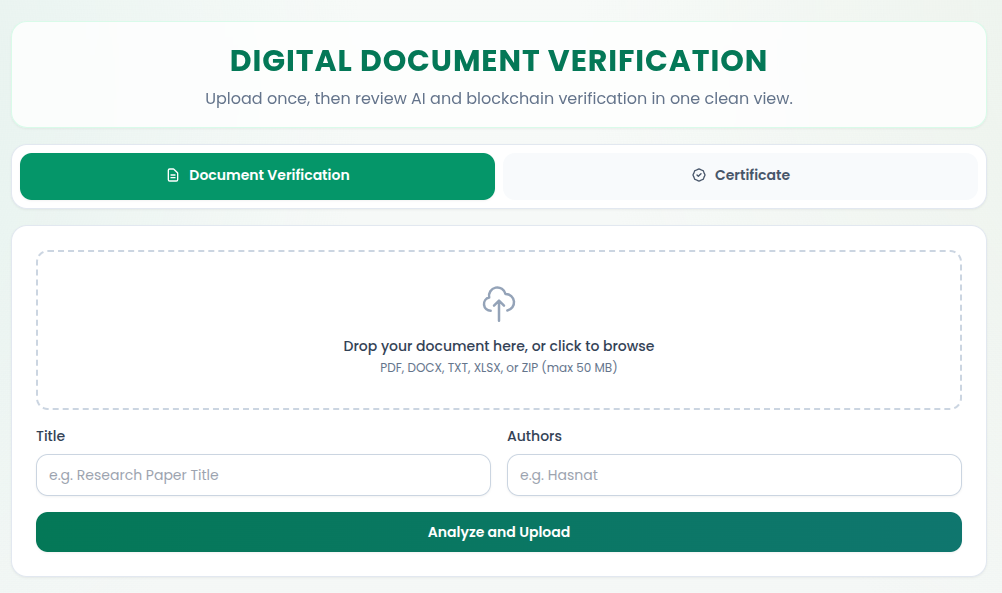
\includegraphics[width=0.8\linewidth]{figures/UI/initial_paper_verification_UI.png}
%             \label{Article or Journal paper verification UI}
%             \caption{Article or Journal paper verification UI}
%         \end{figure}

%         \begin{figure}[H]
%             \centering
%             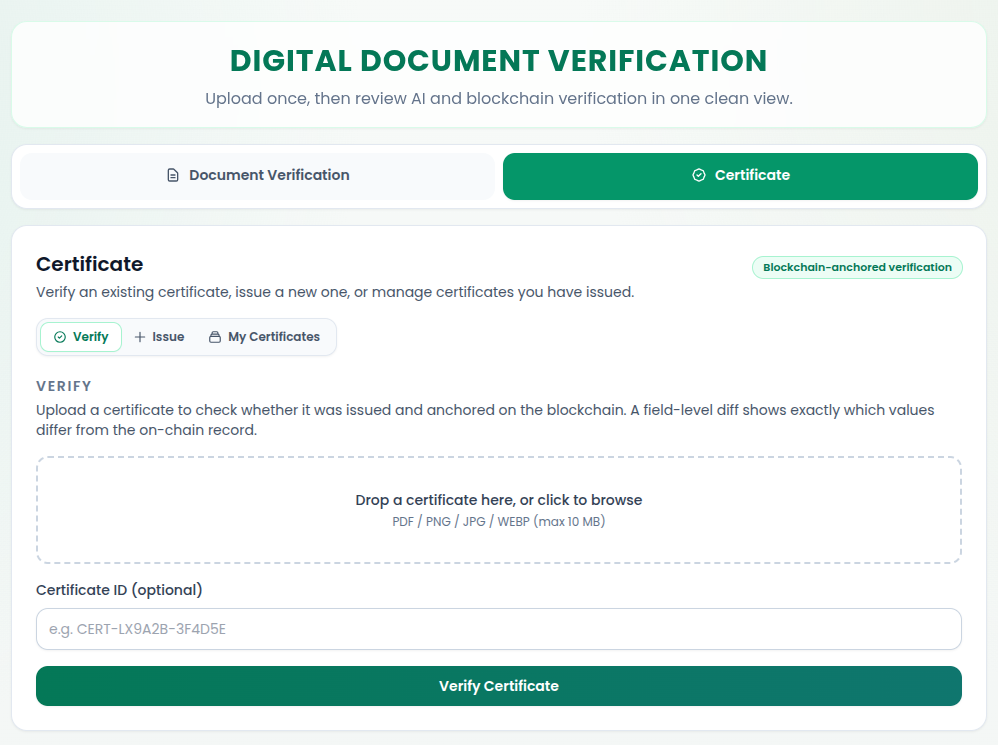
\includegraphics[width=0.8\linewidth]{figures/UI/initail_certificate_verification_ui.png}
%             \label{Certificate verification UI}
%             \caption{Certificate verification UI}
%         \end{figure}
        
%         When results come in, special components show them off. They display stuff like how authentic the document seems, its key parts, and the system's confidence levels. Also, there are visual clues like progress bars and status labels which make it easier for anyone to understand what happened.
%     \subsection{Backend Application Server Module}
%         The backend server handles the main application logic and manages interaction between frontend clients, semantic processors, database systems, and blockchain nodes. It uses an event-driven pattern for async request processing, which keeps resource use efficient during high concurrency.

%         The document submission endpoint accepts multipart form-data containing file uploads and metadata. Upon receipt, the server performs the following sequence of operations:

%         \begin{enumerate}
%             \item File storage in designated upload directory with SHA-256 hash-based naming to prevent naming collisions and facilitate rapid file retrieval.
%             \item Document preprocessing to standardize format and extract text content using optical character recognition (OCR) services for image-based documents.
%             \item Metadata extraction including document dimensions, text statistics and format characteristics.
%             \item Initialization of asynchronous verification workflow, with status stored in the relational database.
%         \end{enumerate}
%         The backend server uses middleware for things like auth, permissions, logging, and error management. Authentication checks a user’s creds before allowing access to protected functions, whereas authorization makes sure they have the right roles to do admin stuff like setting rules or looking at audit logs.

%         Middleware also grabs errors during request processing and turns them into useful HTTP responses for the user, complete with helpful error messages and recovery tips.

%     % \subsection{Semantic Verification Module}
%     % The semantic verification module checks if a document is authentic by analyzing its content. It extracts text from the document and examines it for signs of forgery or manipulation.
    
%     % The module processes documents in steps:
%     %     \begin{enumerate}
%     %         \item Extract text from the document while keeping track of structure and formatting.
%     %         \item Break the text into manageable chunks for analysis.
%     %         \item Check for suspicious patterns including:
%     %         \begin{enumerate}
%     %            \item Terminology inconsistencies: different terms used for the same concept.
%     %            \item Style differences: writing style different from expected for that document type.
%     %            \item Logical errors: contradictions in facts, dates, or sequences.
%     %            \item Missing references: claims without supporting evidence.
%     %            \item Text generation artifacts: patterns typical of AI-generated text.
%     %         \end{enumerate}
%     %     \end{enumerate}
    
    
%     % The module produces a confidence score from 0 to 1 representing the likelihood 
%     % that the document is authentic. Intermediate scores require human review before 
%     % making final decisions.

%     \subsection{Explainable AI Module}
%         The explainable AI module explains why the system made a specific verification decision. Instead of just saying "document is authentic" or "document is suspicious", it shows the evidence supporting that conclusion.
        
%         \begin{figure}[H]
%             \centering
%             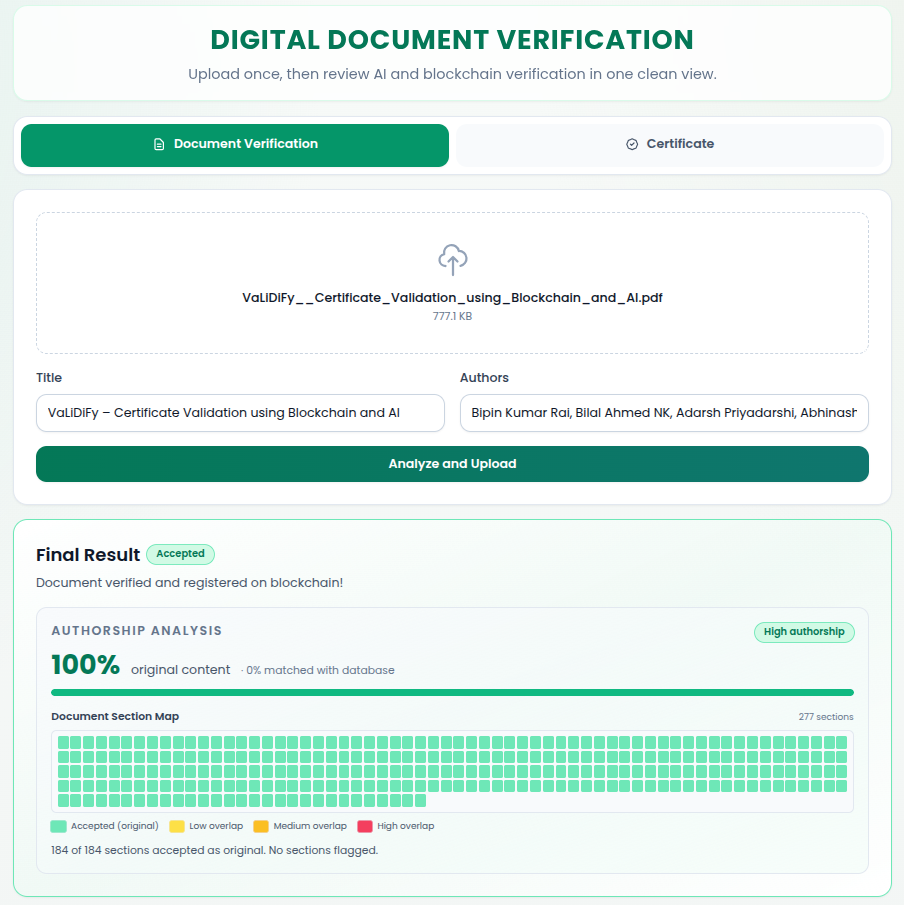
\includegraphics[width=0.8\linewidth]{figures/UI/accepted_paper_ui.png}
%             \label{Article or Journal paper verification UI}
%             \caption{Showing paper is accepted}
%         \end{figure}
        
%         The module identifies which parts of the document most influenced the decision. It highlights text excerpts, metadata characteristics, and document features that contributed most to the final verdict.
        
%         For each verification result, the module generates an explanation containing:
%         \begin{enumerate}
%             \item The final verdict and confidence score
%             \item Specific document excerpts supporting the conclusion
%             \item Key factors ranked by importance
%             \item Confidence bounds showing uncertainty ranges
%             \item Processing steps used to reach the conclusion
%         \end{enumerate}
        
%         This explanation format works for both human reviewers and automated systems. It enables stakeholders to audit the decision and identify potential problems.

%         \begin{figure}[H]
%             \centering
%             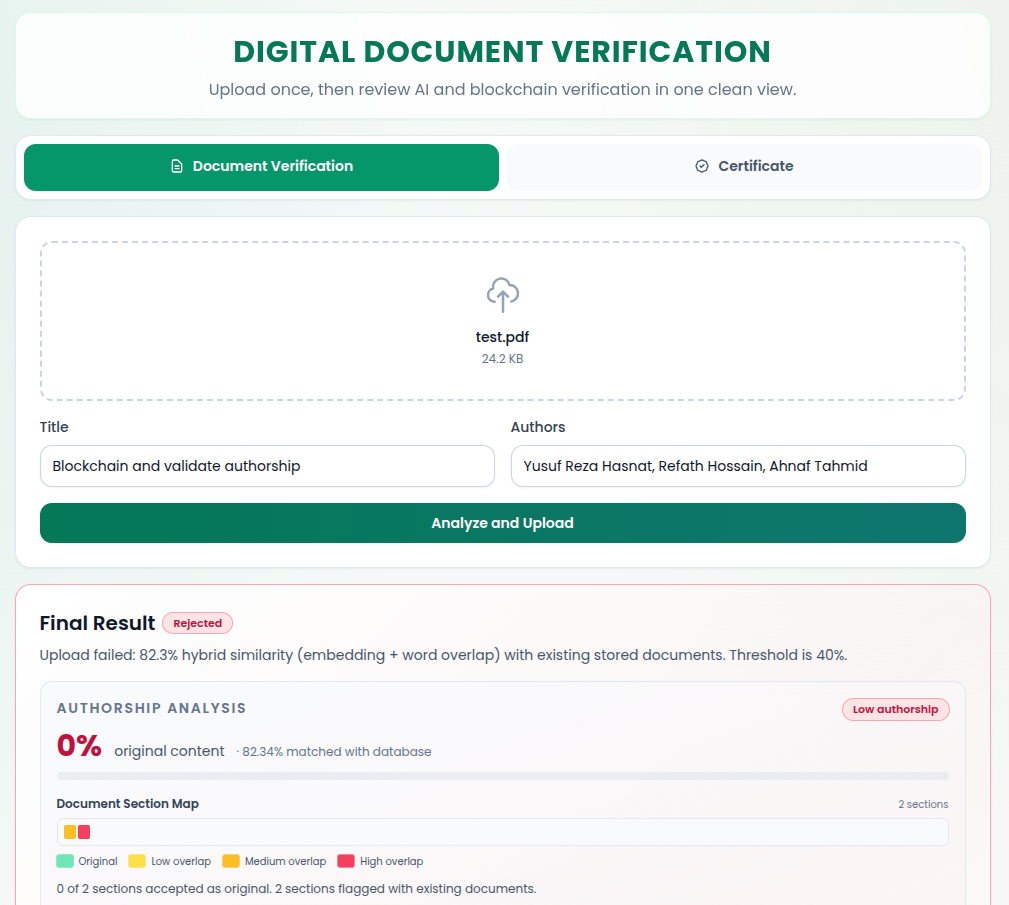
\includegraphics[width=0.8\linewidth]{figures/UI/rejected_paper_ui_1.png}
%             \label{Certificate verification UI}
%             \caption{Showing rejection of a paper}
%         \end{figure}

%         \begin{figure}[H]
%             \centering
%             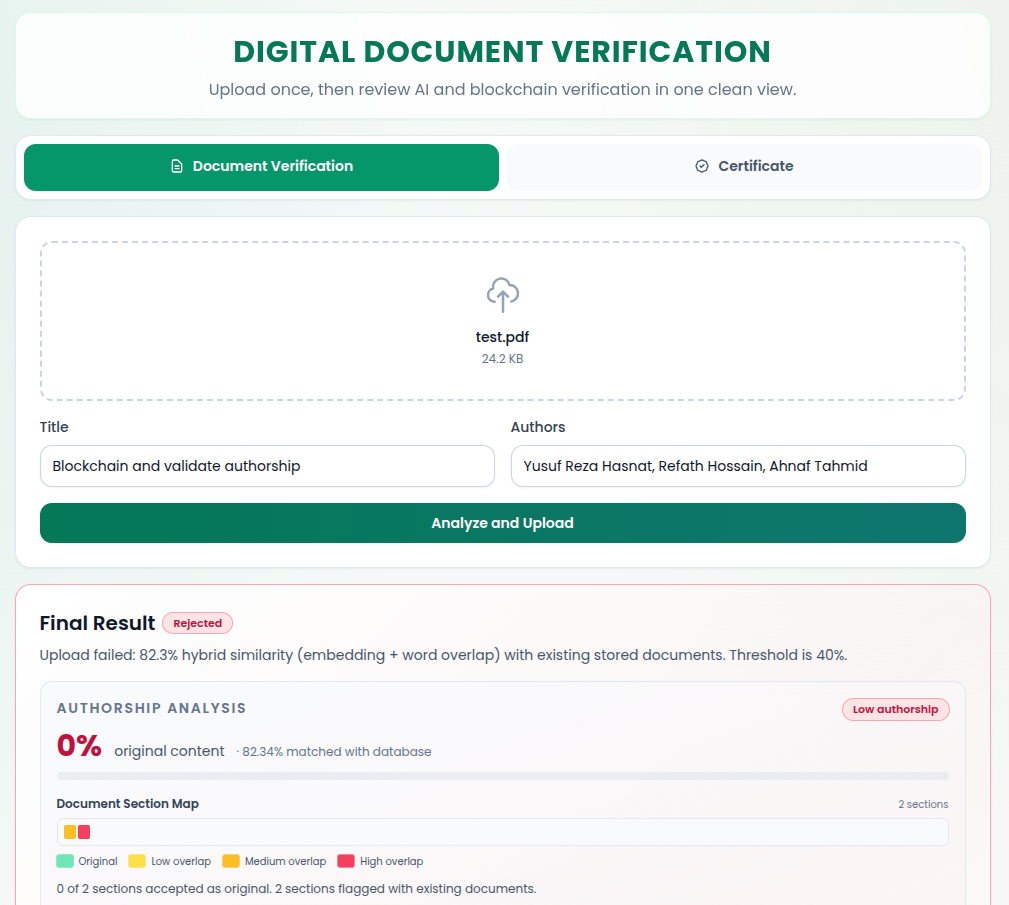
\includegraphics[width=0.8\linewidth]{figures/UI/rejected_paper_ui_1.png}
%             \label{Certificate verification UI}
%             \caption{Explain the rejection of a paper}
%         \end{figure}

%         \begin{figure}[H]
%             \centering
%             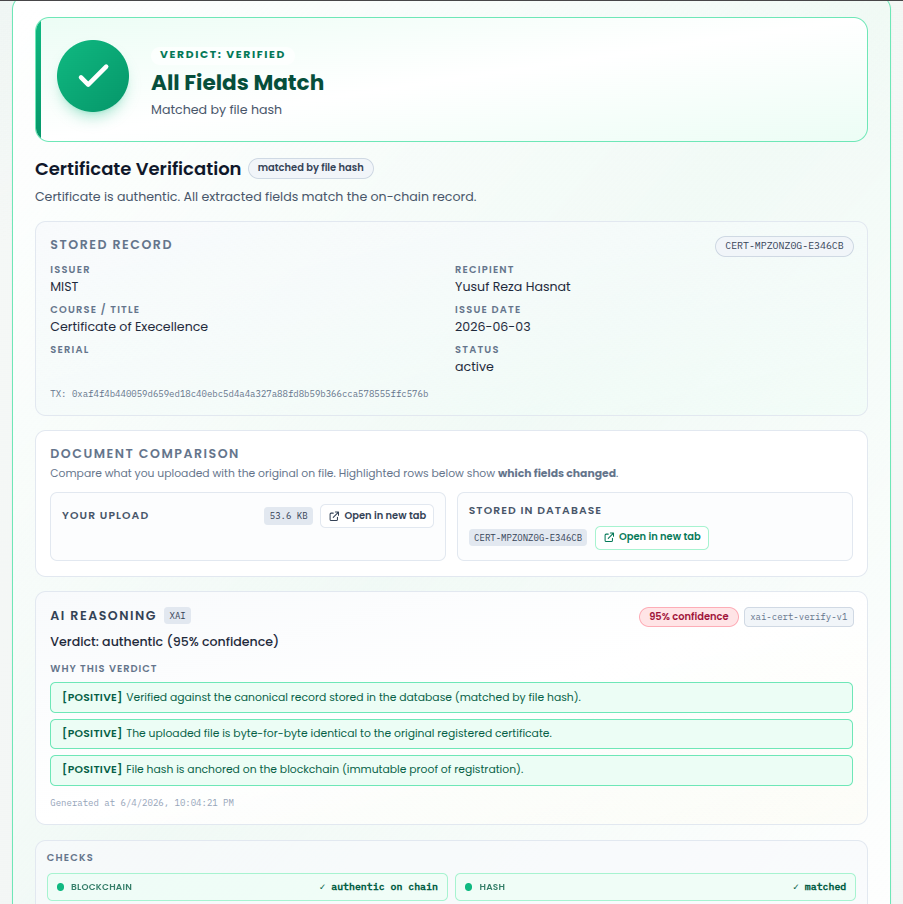
\includegraphics[width=0.8\linewidth]{figures/UI/verify_original_cert.png}
%             \label{Certificate verification UI}
%             \caption{Original Certificate Accept}
%         \end{figure}

%         \begin{figure}[H]
%             \centering
%             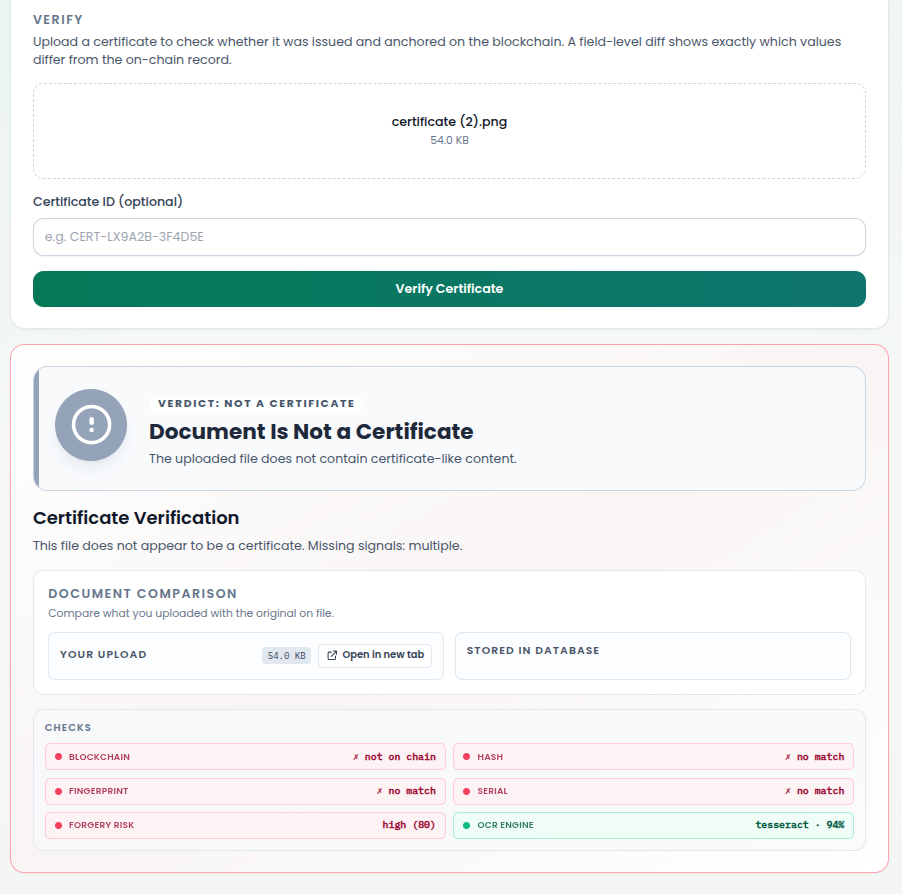
\includegraphics[width=0.8\linewidth]{figures/UI/reject_fake_certificate.png}
%             \label{Certificate verification UI}
%             \caption{Rejecting fake certificate}
%         \end{figure}



%     \subsection{Vector Embedding Service}
%         Vector embeddings convert document text into numerical representations that capture 
%         semantic meaning. These embeddings enable similarity comparisons between documents 
%         by measuring their semantic closeness in vector space.
        
%         The embedding service processes documents through the following steps:
%         \begin{enumerate}
%             \item Text segmentation: divide document into chunks (paragraphs or sentences)
%             \item Encoding: convert each text chunk into a fixed-size numerical vector using 
%                pre-trained embedding models
%             \item Normalization: normalize vectors to standard length for fair comparisons
%             \item Storage: store embeddings in vector database with document references
%         \end{enumerate}
        
%         The embedding service uses transformer-based embedding models that understand 
%         semantic relationships. These models are similar to language models but optimized 
%         for generating meaningful embeddings rather than generating text.
        
%         Embeddings enable several verification capabilities:
%         \begin{enumerate}
%             \item Similarity matching: find other documents with similar content patterns
%             \item Duplicate detection: identify documents suspiciously similar to known forgeries
%             \item Semantic search: retrieve relevant document examples for comparison
%             \item Anomaly detection: identify documents with unusual semantic characteristics
%         \end{enumerate}
        
%         During document verification, the system:

%         \begin{enumerate}
%             \item Generates embeddings for the submitted document
%             \item Queries the vector database for similar documents
%             \item Compares embeddings with known authentic and forged document examples
%             \item Uses similarity scores as additional signals for authenticity assessment
%         \end{enumerate}
        
%         Vector embeddings complement semantic verification by providing geometric similarity 
%         measures. While semantic verification checks for internal inconsistencies, 
%         embeddings assess similarity to reference document sets. Combined, they provide 
%         more robust authenticity assessment.
        
%         The vector database stores millions of document embeddings, enabling rapid 
%         similarity searches even with large document collections. Approximate nearest 
%         neighbor search algorithms enable efficient retrieval of most similar documents 
%         without examining every stored embedding.

%         The system uses a relational database to store operational data about documents, 
%         verification results, and system activity. The database design follows the 
%         structure of the verification workflow.


%     \section{Database Design}
%         The database system was designed to support secure, scalable, and transparent digital document verification within the proposed hybrid framework. Since the system integrates Explainable AI, Optical Character Recognition (OCR), semantic similarity analysis, and blockchain-based verification, the database architecture needed to efficiently manage both structured and unstructured data.

%         PostgreSQL was selected as the primary relational database management system due to its reliability, extensibility, JSON support, and compatibility with vector-based similarity search. The database schema was designed following normalization principles to reduce redundancy while maintaining efficient query performance.
        
%         The architecture consists of four primary entities: Organizations, Certificates, Documents, and Chunks. These entities collectively support certificate issuance, document storage, blockchain verification, OCR processing, and semantic similarity analysis.
        
%         The full SQL implementation of the database schema is provided in Appendix~\ref{appendix:database}

%     \section{Blockchain Setup}
%         The system connects to blockchain networks where verification records are stored. 
%         The blockchain comprises computers (nodes) that maintain copies of all verification 
%         records.
        
%         For development and testing, the system uses local test blockchains. These are 
%         blockchain networks running on the developer's machine, making testing fast and 
%         inexpensive.
        
%         For production, the system can connect to public blockchains like Ethereum. Public 
%         blockchains offer better permanence and decentralization because thousands of 
%         independent nodes maintain copies of the records.
        
%         The system uses a standardized interface to communicate with any blockchain network. 
%         This allows switching between different blockchains without changing the core system code.
        
%         \subsection{Network Configuration and Node Management}
%             The blockchain interface is developed using Hardhat to simulate an Ethereum Virtual environment. Full setup in Appendix~\ref{appendix:hardhat_config}
%             \begin{enumerate}
%                 \item \textbf{Development Network:} Configured locally at http://127.0.0.1:8545 with a custom chain ID of 1337. Gas limits and automatic mining are defined to enable instant transaction confirmation.
%                 \item \textbf{Production Gateway:} Can be pointed to public networks (e.g., Ethereum Mainnet, Polygon, or Arbitrum) by updating the JSON-RPC provider endpoints and deployment configurations.
%             \end{enumerate}

           
%         \subsection{Transaction Management}
                        
%             Transactions are created and signed by the server using the first account initialized by the Hardhat local node. To prevent transaction failures caused by network latency or node connection drops, the backend implements a transaction queue:
%             \begin{enumerate}
%                 \item \textbf{Serialization:} Transactions are built with explicit gas limits to prevent out-of-gas errors.
%                 \item \textbf{Queue Pipeline:} Pending transactions are logged to the database. If a blockchain node becomes unavailable, the system queues submissions and retries them once connectivity is restored.
%                 \item \textbf{Receipt Integration:} When a transaction is confirmed by the network, the backend receives the transaction receipt, extracts the hash and block number, and updates the corresponding record in PostgreSQL.
%             \end{enumerate}

%     \section{Smart Contract Implementation}
%         Smart contracts are programs that run on the blockchain. They store verification records and enforce rules about who can add or view records.
%         \subsection{DocumentRegistry Contract}
%             The main smart contract, called DocumentRegistry, stores document verification records. It maintains mappings between document hashes and verification information. The contract stores:
%             \begin{enumerate}
%                 \item DocumentRecord: contains document hash, owner address, verification timestamp,  and confidence score
%                 \item documentRegistry mapping: maps document hashes to DocumentRecord entries for fast lookup
%                 \item ownerDocuments mapping: tracks which documents belong to each owner
%             \end{enumerate}
%             The contract provides these functions:
%             \begin{enumerate}
%                 \item \textbf{registerDocument(documentHash, score):} Adds a new verification record to the blockchain. Only authorized backend services can call this function. Records the document hash, score, and current timestamp. Broadcasts a DocumentRegistered event so other systems know a new record was added.

%                 \item \textbf{retrieveDocumentRecord(documentHash):} Retrieves verification information for a document hash. Anyone can call this function without permission. Returns the record containing document metadata, owner information, and timestamp.

%                 \item \textbf{verifyDocumentAuthenticity(documentHash):} checks if a specific document hash exists in the registry. Returns true if the document was previously verified, false otherwise. Useful for quick lookups.
                
%             \end{enumerate}
%             The complete Solidity implementation of the smart contract is provided in Appendix~\ref{appendix:smartcontract}.
%         \subsection{Access Control}
%            To protect the integrity of records registered on-chain, access controls restrict write operations while keeping read access open to the public:
%             \begin{enumerate}
%                 \item Authorized Server Execution (Write Interface): Only authorized accounts can send write transactions (like registerDocument or verifyDocument). The backend server uses a private key stored in its environment variables (.env) to sign these transactions.
%                 \item Public Verification (Read Interface): The read-only queries (documentExists, getDocument, and getVerificationStatus) are public and do not require signing keys or gas fees. Any client application can connect directly to the blockchain node to verify a document's status using its hash.
%             \end{enumerate}
    
%     \section{Document Hashing Process}
%         Document hashing produces fixed-length cryptographic fingerprints representing document content. The hashing process ensures that identical documents produce identical hashes, while minimal content modifications produce completely different hashes, detecting unauthorized alterations.
%         \subsection{SHA-256 Hash Computation}
%             The system implements SHA-256 cryptographic hashing, producing 256-bit hash digests. The hashing process operates on complete document byte sequences, ensuring comprehensive content coverage. Hash computation occurs at multiple stages within the verification workflow:

%             \begin{enumerate}
%                 \item Upon document upload, the backend computes document hashes for storage identification and duplicate detection.
                
%                 \item Prior to blockchain registration, content hashes are computed to generate immutable document identifiers for registry entries.
                
%                 \item During verification queries, document hashes enable rapid lookup of existing verification records without requiring full document storage search.
%             \end{enumerate}

%         \subsection{Hash Collision Resistance and Security}
%             SHA-256 is secure because it's really resistant to hash inversions and collisions. Making either of those things happen takes way too much computing power. So, nobody can cheat the system by faking hashes or messing with document verification, at least not anytime soon.
%         \subsection{Hash-Based Document Deduplication}
%             Document hashes help spot previously submitted identical documents. When users upload a document with a matching hash, the system pulls the stored verification results instead of running the whole process again. This speeds things up and lightens the system's workload, especially for duplicates.

